\documentclass[12pt, a4paper]{article}
% Some fancy symbols
\usepackage{textcomp}
\usepackage{stmaryrd}
\usepackage{cancel}

% Some fancy symbols
\usepackage{textcomp}
\usepackage{stmaryrd}


\usepackage{array}

% Math packages
\usepackage{amsmath,amsthm,amssymb, amsfonts, mathrsfs, dsfont, mathtools}
% \usepackage{mathtext}

\usepackage[bb=boondox]{mathalfa}
\usepackage{bm}

% To conrol figures:
\usepackage{subfig}
\usepackage{adjustbox}
\usepackage{placeins}
\usepackage{rotating}



\usepackage{lipsum}
\usepackage{psvectorian} % Insanely fancy text separators!


% Refs:
\usepackage{url}
\usepackage[backref]{hyperref}

% Fancier tables and lists
\usepackage{booktabs}
\usepackage{enumitem}
% Don't indent paragraphs, leave some space between them
\usepackage{parskip}
% Hide page number when page is empty
\usepackage{emptypage}


\usepackage{multicol}
\usepackage{xcolor}

\usepackage[normalem]{ulem}

% For beautiful code listings:
% \usepackage{minted}
\usepackage{listings}

\usepackage{csquotes} % For citations
\usepackage[framemethod=tikz]{mdframed} % For further information see: http://marcodaniel.github.io/mdframed/

% Plots
\usepackage{pgfplots} 
\pgfplotsset{width=10cm,compat=1.9} 

% Fonts
\usepackage{unicode-math}
% \setmathfont{TeX Gyre Termes Math}

\usepackage{fontspec}
\usepackage{polyglossia}

% Named references to sections in document:
\usepackage{nameref}


% \setmainfont{Times New Roman}
\setdefaultlanguage{russian}

\newfontfamily\cyrillicfont{Kurale}
\setmainfont[Ligatures=TeX]{Kurale}
\setmonofont{Fira Code}

% Common number sets
\newcommand{\sN}{{\mathbb{N}}}
\newcommand{\sZ}{{\mathbb{Z}}}
\newcommand{\sZp}{{\mathbb{Z}^{+}}}
\newcommand{\sQ}{{\mathbb{Q}}}
\newcommand{\sR}{{\mathbb{R}}}
\newcommand{\sRp}{{\mathbb{R^{+}}}}
\newcommand{\sC}{{\mathbb{C}}}
\newcommand{\sB}{{\mathbb{B}}}

% Math operators

\makeatletter
\newcommand\RedeclareMathOperator{%
  \@ifstar{\def\rmo@s{m}\rmo@redeclare}{\def\rmo@s{o}\rmo@redeclare}%
}
% this is taken from \renew@command
\newcommand\rmo@redeclare[2]{%
  \begingroup \escapechar\m@ne\xdef\@gtempa{{\string#1}}\endgroup
  \expandafter\@ifundefined\@gtempa
     {\@latex@error{\noexpand#1undefined}\@ehc}%
     \relax
  \expandafter\rmo@declmathop\rmo@s{#1}{#2}}
% This is just \@declmathop without \@ifdefinable
\newcommand\rmo@declmathop[3]{%
  \DeclareRobustCommand{#2}{\qopname\newmcodes@#1{#3}}%
}
\@onlypreamble\RedeclareMathOperator
\makeatother


% Correction:
\definecolor{correct_color}{HTML}{009900}
\newcommand\correction[2]{\ensuremath{\:}{\color{red}{#1}}\ensuremath{\to }{\color{correct_color}{#2}}\ensuremath{\:}}
\newcommand\inGreen[1]{{\color{correct_color}{#1}}}

% Roman numbers && fancy symbs:
\newcommand{\RNumb}[1]{{\uppercase\expandafter{\romannumeral #1\relax}}}
\newcommand\textbb[1]{{$\mathbb{#1}$}}



% MD framed environments:
\mdfsetup{skipabove=1em,skipbelow=0em}

% \mdfdefinestyle{definition}{%
%     linewidth=2pt,%
%     frametitlebackgroundcolor=white,
%     % innertopmargin=\topskip,
% }

\theoremstyle{definition}
\newmdtheoremenv[nobreak=true]{definition}{Определение}
\newmdtheoremenv[nobreak=true]{theorem}{Теорема}
\newmdtheoremenv[nobreak=true]{lemma}{Лемма}
\newmdtheoremenv[nobreak=true]{problem}{Задача}
\newmdtheoremenv[nobreak=true]{property}{Свойство}
\newmdtheoremenv[nobreak=true]{statement}{Утверждение}
\newmdtheoremenv[nobreak=true]{corollary}{Следствие}
\newtheorem*{note}{Замечание}
\newtheorem*{example}{Пример}

% To mark logical parts
\newcommand{\existence}{{\circled{$\exists$}}}
\newcommand{\uniqueness}{{\circled{$\hspace{0.5px}!$}}}
\newcommand{\rightimp}{{\circled{$\Rightarrow$}}}
\newcommand{\leftimp}{{\circled{$\Leftarrow$}}}


% Useful symbols:
\renewcommand{\qed}{\ensuremath{\blacksquare}}
\renewcommand{\vec}[1]{\overrightarrow{#1}}
\newcommand{\eqdef}{\overset{\mathrm{def}}{=\joinrel=}}
\newcommand{\isdef}{\overset{\mathrm{def}}{\Longleftrightarrow}}
\newcommand{\inductdots}{\ensuremath{\overset{induction}{\cdots}}}

% Matrix's determinant
\newenvironment{detmatrix}
{
  \left|\begin{matrix}
}{
  \end{matrix}\right|
}

\newenvironment{complex}
{
  \left[\begin{gathered}
}{
  \end{gathered}\right.
}


\newcommand{\nl}{$~$\\}

\newcommand{\tit}{\maketitle\newpage}
\newcommand{\tittoc}{\tit\tableofcontents\newpage}


\newcommand{\vova}{  
    Латыпов Владимир (конспектор)\\
    {\small \texttt{t.me/donRumata03}, \texttt{github.com/donRumata03}, \texttt{donrumata03@gmail.com}}
}


\usepackage{tikz}
\newcommand{\circled}[1]{\tikz[baseline=(char.base)]{
            \node[shape=circle,draw,inner sep=2pt] (char) {#1};}}

\newcommand{\contradiction}{\circled{!!!}}

% Make especially big math:

\makeatletter
\newcommand{\biggg}{\bBigg@\thr@@}
\newcommand{\Biggg}{\bBigg@{4.5}}
\def\bigggl{\mathopen\biggg}
\def\bigggm{\mathrel\biggg}
\def\bigggr{\mathclose\biggg}
\def\Bigggl{\mathopen\Biggg}
\def\Bigggm{\mathrel\Biggg}
\def\Bigggr{\mathclose\Biggg}
\makeatother


% Texts dividers:

\newcommand{\ornamentleft}{%
    \psvectorian[width=2em]{2}%
}
\newcommand{\ornamentright}{%
    \psvectorian[width=2em,mirror]{2}%
}
\newcommand{\ornamentbreak}{%
    \begin{center}
    \ornamentleft\quad\ornamentright
    \end{center}%
}
\newcommand{\ornamentheader}[1]{%
    \begin{center}
    \ornamentleft
    \quad{\large\emph{#1}}\quad % style as desired
    \ornamentright
    \end{center}%
}


% Math operators

\DeclareMathOperator{\sgn}{sgn}
\DeclareMathOperator{\id}{id}
\DeclareMathOperator{\rg}{rg}
\DeclareMathOperator{\determinant}{det}

\DeclareMathOperator{\Aut}{Aut}

\DeclareMathOperator{\Sim}{Sim}
\DeclareMathOperator{\Alt}{Alt}



\DeclareMathOperator{\Int}{Int}
\DeclareMathOperator{\Cl}{Cl}
\DeclareMathOperator{\Ext}{Ext}
\DeclareMathOperator{\Fr}{Fr}


\RedeclareMathOperator{\Re}{Re}
\RedeclareMathOperator{\Im}{Im}


\DeclareMathOperator{\Img}{Im}
\DeclareMathOperator{\Ker}{Ker}
\DeclareMathOperator{\Lin}{Lin}
\DeclareMathOperator{\Span}{span}

\DeclareMathOperator{\tr}{tr}
\DeclareMathOperator{\conj}{conj}
\DeclareMathOperator{\diag}{diag}

\expandafter\let\expandafter\originald\csname\encodingdefault\string\d\endcsname
\DeclareRobustCommand*\d
  {\ifmmode\mathop{}\!\mathrm{d}\else\expandafter\originald\fi}

\newcommand\restr[2]{{% we make the whole thing an ordinary symbol
  \left.\kern-\nulldelimiterspace % automatically resize the bar with \right
  #1 % the function
  \vphantom{\big|} % pretend it's a little taller at normal size
  \right|_{#2} % this is the delimiter
  }}

\newcommand{\splitdoc}{\noindent\makebox[\linewidth]{\rule{\paperwidth}{0.4pt}}}

% \newcommand{\hm}[1]{#1\nobreak\discretionary{}{\hbox{\ensuremath{#1}}}{}}


\graphicspath{{res/}}


\title{Заметки практики по матанализу \\(самые разные семестры)} 

\author{
  \vova
  \and
  {Семёнова Ольга Львовна (препод)}
}

\date{\today}



\begin{document}
  \tittoc


  Здесь можно вспомнить, чем мы всё это время занимались на практике.
  
  «Стенограмма» практик в виде серии фотографий доски (насколько возможно оперативных) есть в телеграм «чатике с домашкамм» начиная с этого сообщения:
  \url{https://t.me/c/1512041988/198}.

  В этом же документе содержится список методов, подходов и трюков,
  которые мы учимся применять на практике.

  Крайне полезного освежать его в памяти перед контрольной по отношению к актуальной теме, 
  а также в любой момент по отношению к давнему материалу.

  Контрибьютинг всячески приветствуется, 
  благо на Github делать это максимально удобно.
  Если вы решили, например, в какой-то момент 
  пролистать свой конспект и вспомнить былое — 
  добавьте в этот конспект то, чего нет здесь — 
  помогите товарицам. 
  Или, если что-то написанное здесь настолько вопиюще неверное, 
  что режет ваши глаза и вызывает желание как можно быстрее это пофиксить — вперёд.

  Насчёт технических деталей — в README описано по шагам, 
  что надо установить, чтобы компилировать конспект у себя на компьютере,
  однако ничего не мешает дописать сюда в обычном текстовом редакторе 
  нечто отдалённо напоминающее латех и послать Pull Request 
  — я исправлю, если что-то не будет компилироваться.


  Конспект организован по темам, в том порядке, в котором мы их проходим на практиках.
  Кроме того, примерно расставлены разделения, 
  где заканчивается предыдущая практика и начинается следующая,
  но могут быть неточности, так как отдаётся приоритет организации по темам.

  На данный момент такая картина готовности тем:

  \begin{itemize}
    \item Пределы — почти ничего
    \item Производные — совсем мало
    \item Интегралы — довольно полно, но тезисно
    \item Числовые ряды — вообще ничего
    \item Функциональные ряды — подробно
    \item Функции нескольких переменных — сами практики в процессе
  \end{itemize}

\section{Пределы}

  \subsection{Таблица эквивалантности}
  Отличная ссылка на таблицу эквивалентности с нужными доказательствами: 
  \url{http://mathserfer.narod.ru/node22.html}

  Альтернативный вариант:
  \url{https://ib.mazurok.com/2013/05/19/table-equ/} 


\section{Дифференциальное исчисление одной переменной}

  \subsection{Испольозвание первой и второй производной для построения картины функции и её поведения 
    у себя в голове и последующего её перенесения на бумагу}

    А именно: 

    \begin{itemize}
      \item Находим область определения
      \item Смотрим поведение на границах области определения (значения, предел, асимптоты)
      \item Первая производная $\Longrightarrow$ делаем вывод о промежутках возрастания/убывания, экстремумах
      \item Вторая производная $\Longrightarrow$ выпуклость, точки перегиба
    \end{itemize}

    \subsection{Оптимизация функций через поиск и проверку критических точек с помощью производной, например, параметры геометрических фигур}

\section{Интегральное исчисление одной переменной}

  \subsection{Символьное вычисление неопределённых интегралов}

    \begin{itemize}
      \item Таблица интегрирования основных элементарных функций
      \item Базовые приёмы интегрирования: замена переменной, ингегрирование по частям
      \item Тригонометрические и гиперболические подстановки
      \item Интегрирование по индукции, если функция содержит целочисленный параметр
      \item Сведение интеграла самого к себе, например, $\sqrt{x^2 + a^2} \rightarrow \frac{t}{\sqrt{x^2 + a^2}} t + \ldots \rightarrow$ по частям.
      \item Выделение полного квадрата под корнем или не под корнем в знаменателе, избавление от линейного члена
      \item Если есть подвыражения вида $x + a$, замена переменной $t = \frac{1}{x + a}$
      \item Выделение в числителе производной знаменателя, например, \url{https://ru.wikipedia.org/wiki/%D0%98%D0%BD%D1%82%D0%B5%D0%B3%D1%80%D0%B8%D1%80%D0%BE%D0%B2%D0%B0%D0%BD%D0%B8%D0%B5_%D1%80%D0%B0%D1%86%D0%B8%D0%BE%D0%BD%D0%B0%D0%BB%D1%8C%D0%BD%D1%8B%D1%85_%D1%84%D1%83%D0%BD%D0%BA%D1%86%D0%B8%D0%B9#%D0%98%D0%BD%D1%82%D0%B5%D0%B3%D1%80%D0%B8%D1%80%D0%BE%D0%B2%D0%B0%D0%BD%D0%B8%D0%B5_%D0%B4%D1%80%D0%BE%D0%B1%D0%B5%D0%B9_%D0%B2%D0%B8%D0%B4%D0%B0_%7F'%22%60UNIQ--postMath-0000007E-QINU%60%22'%7F}.
      \item Рациональные функции: разложение на простейшие, далее элементарно, больше второй степени не получится
      \item Функции вида $R\left(x, \sqrt[N]{\frac{\alpha x + \beta}{\gamma x + \delta}}\right)$ через замену переменной на весь корень.
      \item Подстановки Эйлера: $R\left(x, \sqrt{ax^2 + bx + c}\right)$. В зависимости от коэффициентов нужно выбрать правильное $t$. 
      Случаи могут быть пересекаться. Для функции подходят все те случаи, под условия которых она подходит:
      \begin{enumerate}
        \item При $a > 0$: ${\sqrt {ax^{2}+bx+c}}=\pm t\pm {\sqrt {a}}x$
        \item При $c > 0$: ${ {\sqrt {ax^{2}+bx+c}}=\pm t\pm {\sqrt {a}}x}$
        \item При наличии двух вещественных корней: ${{\sqrt {ax^{2}+bx+c}}=\pm t(x-\lambda )}$, где $\lambda$ — один из корней
      \end{enumerate}
      \item Интегрирование дифференциальных биномов
      
      \begin{equation}
        \int x^{m}(a+bx^{n})^{p}\,\mathrm{d}x = \begin{bmatrix} z = x^n \\ \mathrm{d}x = \frac{1}{n} z^{\frac{1 - n}{n}} \mathrm{d}z \end{bmatrix} = \frac{1}{n} \int z^{\frac{m}{n} + \frac{1 - n}{n}}(a+bz)^{p}\,\mathrm{d}z
      \end{equation}

      \begin{equation}
        q = \frac{m}{n} + \frac{1 - n}{n}
      \end{equation}
      
      3 случая интегрируемости:
      \begin{enumerate}
        \item $p \in \sZ, q = \frac{M}{N}$: $t = z^{\frac{1}{N}}$, выражаем получаем $R(t)$. Профит.
      \end{enumerate}
      \item Тригонометрические подстановки в рациональных функциях $R(\cos x, \sin x)$:
      \begin{itemize}
        \item Если $R(-\cos x, \sin x) = -R(\cos x, \sin x)$ (нечётно относительно $\cos$), можно $t = \sin x$
        \item Если $R(\cos x, -\sin x) = -R(\cos x, \sin x)$ (нечётно относительно $\sin$), можно $t = \cos x$
        \item Если $R(-\cos x, -\sin x) = R(\cos x, \sin x)$ (чётно по обеим вместе), можно $t = \tg x$
        \item Наконец, универсальное, $t = \tan \frac{x}{2}$ работает всегда, через неё легко выражаются $\sin, \cos, \frac{\mathrm{d}t}{\mathrm{d}x}$.
      \end{itemize}
      \item Похожая шняга получается и с $R(ch\, x, sh\, x)$
      \item Линейное выражение числителя через знаменатель и его производную, решение системы уравнений
    \end{itemize}
  
  \subsection{Определённые интегралы}
  
  \begin{itemize}
    \item Формула Ньютона-Лейбница
    \item Замена переменной, если особые точки не появляются, ничего не портит
    \item При интегрировании по частями надо смотреть, чтобы сумма частей имела смысл в $\overline{\sR}$.
  \end{itemize}



    
  \subsection{Несобственные интегралы}

  \begin{itemize}
    \item Взятие предела для несобстыенных интегралов, если получается сделать это в явном виде
    \item Рассмотрение «особенных» точек, их может быть несколько
    \item Анализ сходимости: сначала проверяем абсолютную, потом относительную
    \item Критерий Коши (если любое значение после некоторого $A$ не превышается ни на каком промежутке в $\sR$).
    \item Разбиение промежутка на несколько
    \item Использование асимптотического анализа для определения абсолютной сходимости
    \item Дирихле и Абель — позволяют сделать вывод об абсолютной сходимости функции, представленной произведения
      \begin{itemize}
        \item Дирихле: первая имеет ограниченную первообразную, вторая — монотонно → 0, тогда сходится
        \item Абель: первый интеграл сходится, вторая монотонна и ограничена, тогда тоже сходится
      \end{itemize}
    \item Разложение подинтегральной функции в ряд Тейлора: спросить у кого-то
  \end{itemize}


\section{Числовые ряды}

% TODO
  

\section{Функциональные ряды}

\ornamentheader{Практика 5 сентября 2022}

Фотоотчёт за практику: \url{https://t.me/c/1512041988/198}

Pro tip: для $\alpha < \frac{\pi}{2}$ — $\sin \alpha > \alpha \frac{2}{\pi}$ за счёт выпуклости.

\subsection{Исследуем равномерную сходимость}

\begin{itemize}
	\item Если можем посчитать «колебание» (супремум отколнеиня на всём множестве $E$ при фиксированном $n$), 
  то проанализируем, стремится ли оно к нулю при $n \to \infty$.
	\item Признак Вейерштрасса (мажорантная сходимость для рядов): находим равномерную норму каждого члена, если ряд норм сходиться, то анализируемый ряд — тоже.
	\item Критерий Больцано-Коши (равносильно равномерной сходимости). Сходимость в себе, работает для
	\item Признак Дирихле (равномерная сходимость ряда произведений). У одного частичные суммы \textbf{равномерно огранчиены}, другой стремится к нулю и монотонен по $n$ с некоторого номера при каждом фиксированном $x$. 
  (Теперь везде не забываем добавлять «равномерно»).
  \item Признак Абеля (равномерная сходимость ряда произведений). 
  Тут у первого частичные суммы должны быть \textbf{не равномерно \textit{огранчиены}, а равномерно \textit{сходиться}}, 
  но зато второму достаточно просто быть равномерно ограниченным (и всё ещё монотонным).
  \item Следствие: Лейбниц — сумма знакопеременного, монотонно равномерно сходящегося к 0 ряда со знакочередованием ряда — равномерно сходится.
\end{itemize}

Ещё pro tip: 

\begin{gather}
  \left| \sum_{k = 1}^N \sin {k\alpha} \right| \leqslant \frac{1}{\left| \sin {\frac{\alpha}{2}} \right|} \\
  \left| \sum_{k = 1}^N \cos {k\alpha} \right| \leqslant \frac{1}{\left| \sin {\frac{\alpha}{2}} \right|}
\end{gather}

\subsection{Доказывем отсутствие равномерной сходимости}

Если не сходится поточечно где-то, рассматривать не интересно.

\begin{itemize}
  \item Не на компакте: если замыкание не сходится даже поточечно (на границах)
  \item Если не выполняется хотя бы одно необходимое условие из секции \ref{Свойства равномерно сходящихся} 
  при выполнении остальных предпосылок теоремы
  \item Если можно посчитать в явном виде
  \item Можно оценить остаток через интеграл, если есть монотонность по $n$ и момент, с которой она начинается, не зависит от $x$ — 
  и сказать через него, что найдётся $\varepsilon$, что для любого $n$ найдётся плохой $x$.
  \item Можно сделать то же через критерий Больцано-Коши.
\end{itemize}


\ornamentheader{Практика 12 сентября 2022}

Фотоотчёт за практику: <отсутствует>.


\subsection{Свойства равномерно сходящихся}\label{Свойства равномерно сходящихся}

При равномерной сходимости можно производить перестановку пределов, 
из неё получаем возможность заключить непрерывность предела, 
получаем перестановочность интегрирования и дифференцирования.

Однако это всё получается и при более вольных условиях, но они более сложные, мы их не изучали.



\ornamentheader{Практика 19 сентября 2022}

Фотоотчёт за практику: \url{https://t.me/c/1512041988/208}.


\subsection{Степенные ряды}\label{Степенные ряды}

Ряды вида $\sum_{i = 1}^\infty c_i (z - z_0)^i$.

Умеем искать радиус сходимости 
(это шар, внутри гарантированно сходится, снаружи — не менее гарантированно расходится, 
а на границе — надо думать, анализировать дальше).

\begin{itemize}
  \item Коши (база, работает всегда): ${\displaystyle R = \frac{1}{\limsup_{n \to \infty} \sqrt[n]{|c_n|}}}$
  \item Даламбер (иногда работает и он, если существует): ${\displaystyle R = \lim_{n \to \infty} \left|\frac{c_{n}}{c_{n + 1}}\right|}$
\end{itemize}

Потом можем использовать степенные ряды как составные части для анализа произвольных рядов.

Раскладываем в ряд Тейлора:

Разложить можем, чтобы в пределе все производные совпадали, но когда она будет совпадать с самой функцией на каком-то промежутке?

Оказывается, что достаточно комплексной дифференцируемости в $B_R(z_0)$ 
— тогда существует единственный набор коэффициентов степенного ряда с заданным центром, 
с пределом которого функция совпадает — и коэффициенты тогда находятся через Тейлора.

Note: для комплексной дифференцироемости выполняются все естественнные свойства обычной: 
замкнутость относительно арифметических операций, дифференцируемость элементарных функций, производная локальной обратимой функции и т.д.

Разложение элементарных функций в степенной ряд было на доске..

Как раскладывать в степенные ряды?

\begin{itemize}
  \item Честно, через производные по Тейлору
  \item Раскладывать в произведение — перемножать ряды
  \item В круге сходимости дифференцировать можно почленно — 
  замечаем, что ряд является интегралом чего-то хорошего — и дифферегнцирем его ряд.
  \item Аналогично — если является производной чего-то хорошего
  \item Можно пользоваться тем, что сумма ряда равна функции в круге сходимости. Например, 
  \begin{equation}
    \frac{1}{x - x_0} = \frac{1}{-x_0}\left(\frac{1}{1-\frac{x}{x_0}}\right) = -\frac{1}{x_0} \sum_{k = 0}^\infty \left(\frac{x}{x_0}\right)^k
  \end{equation}
\end{itemize}


\ornamentheader{Практика 26 сентября 2022}

Фотоотчёт за практику: \url{https://t.me/c/1512041988/216}


Если у нас уже есть ряд, и надо проанализировать, какую функцию он описывает или его свойства.

\begin{itemize}
  \item Для анализа схоимости можно посмотреть на коэффициент, как всегда.
  \item Можно применить метод божественного озарения и, например, продифференцировать, умножить на какую-то сдвигающую скобку и заметить, 
  что получилось нечто содержащее исходный ряд, получив диффуру…
\end{itemize}

Признак сходимости обычных, положительных рядов, обобщающий признак Д'Аламбера — признак Гаусса:

\begin{equation}
  \frac{a_n}{a_{n+1}} = \lambda + \frac{\mu}{n} + O\left(\frac{1}{n^{1 + \varepsilon}}\right), \varepsilon > 0
\end{equation}

Тогда при $\lambda > 1$ — сходится, если $\lambda < 1$ — расходится, 
иначе (при $\lambda = 1$) — $\mu > 1$ — сходится, $\mu \leqslant 1$ — расходится.


\section{Функции нескольких переменных}

\subsection{Берём пределы}

Какие механизмы?

\begin{itemize}
  \item По Коши/окрестностям: для окрестности результатов найдётся окрестность аргументов, такая что каждый студент знает, какая.
  \item По Гейне — вдоль любой последовательности, стремящейся к $x_0$ по $D \\ \{x_0\}$ $f(x_n) → A$
  \item Эквивалентно (тривиально — про Коши) — $\sup_{x \in \overset{.}{V}_\delta (x_0) \cap D} \left| f(x) - A \right| \underset{\delta → 0}{\longrightarrow} 0$
\end{itemize}



\subsection{Разница между повторным и двойным пределом}

У «хороших» функций, конечно, их существование эквивалентно и они равны. Наверное, Липшицевости достаточно.
Также, (по теореме о двойном пределе) если существует конечный или бесконенчный двойной предел, 
а также для каждого фиксированного $x'$ в окрестности существует конечный предел сужения $\varphi(y) = f(x', y)$, то пределы равны.
Но вообще могут быть такие варианты:

\begin{itemize}
  \item Двойной существует, а $\forall x \neq x_0$ не существует даже внутрення часть повторного предела
  \item Может не сущетствовать двойной, и это можно доказать по Гейне, показав две последовательности, вдоль которых пределы не равны
  \item Может стремиться к $0$ вдоль любого луча от 0 к ∞, но не быть бесконечно малой на $x, y → +∞$. Например, $f(x,y)=x^2 e^{-(x^2-y)}$
\end{itemize}

\begin{figure}[h!]
  \centering
  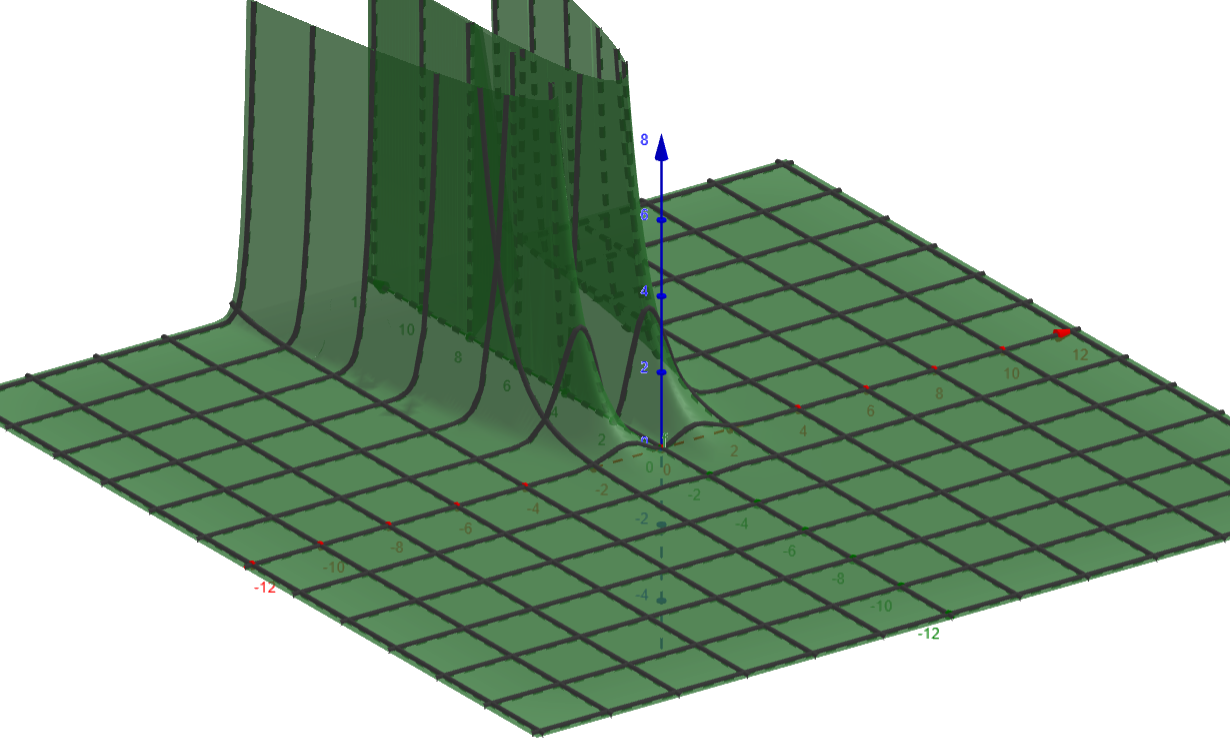
\includegraphics[width=\textwidth]{res/weird_func_no_lim.png}
  \caption{Та самая $f(x,y)=x^2 e^{-(x^2-y)}$}
  \label{fig:no_lim}
\end{figure}
\FloatBarrier 

Примеры c разбором есть в фотоотчёте практики 26.09: \url{https://t.me/c/1512041988/216}. 

\ornamentheader{Практика 10 октября 2022}

Фотоотчёт за практику: \url{…}

Как доказать существование предела функции, например, на $+\inf, +\inf$?

В определении предела фигурирует окрестность точки $+\inf, +\inf$, то есть

\begin{equation}
  \begin{cases}
    x > \varepsilon \\
    y > \varepsilon
  \end{cases}
\end{equation}

В отличие от просто $||x, y|| → \inf$, когда .

\begin{itemize}
  \item Нужно оценить супремум отклонения от предела при $x > \varepsilon, y > \varepsilon$.
  \item К полянрым координатам и оценить супремум по некоторой части сферы (для $+\inf, +\inf$, казалось бы — по $\varphi \in (0, \pi/2)$). 
  Но по идее, это будет корректно, так как там $x$ может быть сколь угодно малым. Наверное, надо сузить угол до компактного подмножества $[\alpha, \beta] \subset (0, \pi/2)$.
  И оценить зависимость {супремума по $\varphi$} от $r$.
  Особые извращенцы будут искать супремум через Лагранжа.
\end{itemize}

\subsection{Дифференцирование, частные производные}

Дифференцируема $\isdef$ представима в виде $f(x_0) + A h + o(|h|)$, 
где $A$ — линейный оператор ($A \in \operatorname{Hom} (\sR^n → \sR^m)$).
Частная производная — производная направлению вектора-орта.

Иногда вектор частных производных равен вектору производному оператора. 

Есть необходимое и достаточное условия.

\begin{theorem}
  [Базированная теорема о производных]
  У нормальных функций всё будет нормально.
\end{theorem}

Если быть точнее — для дифференцируемости достаточно сущетствования в окрестноти и непрерывности в точке частных производных по каждой переменной.
Но не необходимо, так как, например, у функции $f(x, y) = \begin{cases}
  x^2 + y^2, \quad (x \in \sQ) \operatorname{xor} (y \in \sQ) \\
  0, \quad \mathrm{otherwise}
\end{cases}$ частные производные вообще не определены ни в каких точках кроме нуля, что уж там говорить о непрерывности.

А для равенства частных производных по разным перестановкам одной и той же последовательности переменных
достаточно (но не необходимо) существования и непрерывности всех \textit{рассматриваемых} частных производных в окрестности.
(Фактически, в теореме было про $r$ раз непрерывную дифференцируемость, то есть вообще по любой последовательности из $r$ переменных).


Как искать частные производные?
Если функция представлена в виде композиций элементарных функций, считаем по формулам, 
фиксируя остальные переменные — воспринимая их как параметры.

Если мы уже посчитали частные производные по всем переменным, 
то проверить дифференцируемость самой функции можно так:

\begin{equation}
  \frac{f(x_0 + h) - f(x_0) - \langle \nabla f, h \rangle}{\lVert h \rVert} → 0
\end{equation}

Но вообще — частная производная всё ещё может сущетвовать, 
даже если по формулам посчитать не получается (формулы-то применимы только там, где всё определено).
Если нет — тогда можем находить их как производные по направлению. Пример:

\begin{equation}
  f(x, y) = \sqrt[3]{xy}
\end{equation}

\begin{equation}
  f'_x(0, 0) = \lim_{\Delta x → 0} \frac{f(\Delta x, 0) - f(0, 0)}{\Delta x} = \lim_{\Delta x → 0} \frac{0}{\Delta x} = \lim_{\Delta x → 0} 0 = 0
\end{equation}

Попробуем применить критерий выше: вдруг этот градиент $(0, 0)$ — и есть производная?

\begin{equation}
  \frac{\sqrt[3]{xy} - 0 - 0}{\sqrt{x^2 + y^2}} →? 0
\end{equation}

Для $x = y$ — стремится к бесконечности, хотя по лучу $x = 0$ или $y = 0$ и ноль, ни о каком стремлении к нулю говорить не приходится.

Для более сложных функций можно представлять их как композицию, заводя переменную для одной из её частей.

Например,

\begin{equation}
  u = \frac{x}{\sqrt{x^2 + y^2}}, u'_{x, y} — ?, u'_{xx, xy, yy} — ?
\end{equation}
(в нижних индексах через запятую — все частные производные, которые требуется найти).

Обозначим $r = \sqrt{x^2 + y^2}, u = r^{-1} x$.

Находим $r'_{x}, r'_{y}$. Тогда $u'_x = (r^{-1})'_x x + r^{-1} \cancelto{1}{x'_x} = …$


Если у нас какая-то большая функция, то частная производная композиции выражается через сумму 
— как элемемент произведения матриц Якоби.

Хозяйке на заметку: $\mathrm{d}\left(\frac{x}{y}\right) = \mathrm{d}\left(\frac{y\mathrm{d}x - x\mathrm{d}y}{y^2}\right)$.

Ещё на заметку: важно отличать $d^2t$ от $dt^2$ (последнее является обозначением для $(dt)^2$).

Первое — второй дифференциал функции (для независимой переменной — это просто ноль, для них никто так не пишет).
Второе — приращение переменной, возведённой в квадрат.

Как искать полные дифференциалы разных порядков?

Можно воспользоваться определением, возникшим из Тейлора — там сумма по всем мультииндексом $k$ порядка $l$.

Для двухмерной переменной достаточно перебирать в суммировании степень вхождения приращения одной из переменных:

\begin{equation}
  \d^n  f = \sum_{k = 0}^{n} 
  \frac{n! f'_{x^k y^{n - k}} } {k! (n - k)!} (\d x)^k (\d y)^{n - k}
\end{equation}

Например, $\d f = f'_x \d x + f'_y \d y$, 

$\d^2 f = f''_{x^2} \d x^2 + 2 f''_{xy} \d x \d y + f''_{y^2} \d y^2$

Но на практиках матанализа дифференциалы первого-второго порядка так не считают, а 
в «символьном» виде, имея полный дифференциал предыдущего порядка и применяя втупую формулу дифференцирования, получают желаемую формулу.

При этом первый дифференциал рассматривают как отображение с той же сигнатурой, что и исходная функция,
считая, что $\d x_i$ берётся то же самое.

Причём 

\begin{multline}
  \d(g(x, y)\d x + h(x, y)\d y) = (g(x, y) \d(\d x) + \d g(x, y) \d x) + (h(x, y) \d(\d y) + \d h(x, y) \d y) = \\
  \begin{bmatrix}
    \d(\d x) = \d^2 x = (\d x)'_x \d x + (\d x)'_y \d y = 0 ← \d x = \mathrm{const\ everywhere} \Rightarrow (\d x)'_x = 0 \\
    \d x \d x = (dx)^2 \eqdef dx^2
  \end{bmatrix} = \\
  \d g(x, y) \d x + \d h(x, y) \d y = (g'_x \d x + g'_y \d y) \d x + (h'_x \d x + h'_y \d y) \d y
\end{multline}

Частные производные функций $g$ и $h$ считаем самостоятельно.
Иногда получится, что какие-то из слагаемых нули, когда что-то не зависит от чего-то.
И потом приведём подобные слагаемые (например, $\d x \d y = \d y \d x$).

Всё это работатет для независимых переменных. 
Но рассмотрим хитрую композицию:

\begin{equation}
  u = f(\frac{x}{y}, \frac{y}{z})
\end{equation}

И мы считаем, что знаем «всё, что нужно» про функцию $f$.

Хотим найти полные диффенерциалы $\d u, \d^2 u$ (полагая $x, y$ независимыми переменными).

И тут у нас получается, что $\d^2 s \neq 0$, так как это более не независимая переменная, а функция.

Так что теперь:

\begin{equation}
  \d^2 u = f''_{s^2} \d s^2 + (f''_{st} + f''_{ts}) \d s \d t + f''_{t^2} \d t^2
  + f'_s \d^2 s + f'_t \d^2 t
\end{equation}

Где $\d^2 s$ — это квадратичная форма (если замена, например, была линейная, она обнуляется).

То есть при $s = \alpha x + \beta y$:
$\d s = \alpha \d x + \beta \d y$, тогда:

\begin{equation}
  \d^2 s = \d^2 x s''_{x^2} + 2 \d x \d y s''_{xy} + \d^2 y s''_{y^2}
\end{equation}

И здесь второе слагаемое уже не обнуляется, и в результате получается не ноль, в отличие от нехависимых переменных.


\ornamentheader{Практика 17.10.2022}

\subsection{Дифференцируем неявно заданные ображения}

Простые равенства дифференцировать нельзя, только тождества 
(равенство должно выполняться в окрестности, чтобы все производные совпадали — они обладают свойством лоакльности, но требуют, чтобы точка 
\sout{была точкой сочленения… кхм} внутренней).

Например, $F(x + y + z, x^2 + y^2 + z^2) = 0$, найти $\frac{\partial^2 z}{\partial x \partial y}$.

\subsection{Дифференцируем системы-неявно заданные отображения}

Фактически — это всё ещё неявные отображения, просто со значениями в $\sR^{n + m}$, где .

Мы можем захотеть выразить дифференциал какого-то порядка одной части через дифференциалы других 
(ну или найти производные одних по другим) — из предположения, что вторая часть — взяты за независимые переменные.

«Инвариантность дифференциалов первого порядка относительно изменения зависимых и независимых переменных»:
то есть не важно, какие переменные выбраны за независимые, дифференциалы удовлетворяют одному и тому же отношению.
Например, $\psi(x, y, z) = 0$; $z = \varphi(x, y)$ — неявное отображение, $dz = \varphi'_x dx + \varphi'_y dy$ — соотношение дифференциалов. 
Если будет $x = \xi(y, z)$ удовлетворяет — тому же самому неявному отображению, 
но теперь зависимая переменная — $x$, то соотношение $\d x = \xi'_y \d y + \xi'_z \d z$ — будет то же самое.
(из теоремы о неявном отображении $\varphi^{\prime}(x)=-\left.\left(\Phi_y^{\prime}(x, y)\right)^{-1} \Phi_x^{\prime}(x, y)\right|_{y=\varphi(x)}$)


А вот для дифференциалов высшего порядка — такого нет. Дифференциалы высших порядков от зависимой переменной могут быть ≠ 0.
Например

\ornamentheader{Практика 24.10.2022}

Параметризация сферы через два угла:
// TODO


\section{Замена переменной в дифференциальных уравнениях}

Если хотим взять за переменную $y$ вместо $x$, нужно выразить $y^{(n)}$ через $x^{(k)}$ и, возможно, $y$.
Раньше искали $f(x) = y$, теперь будем $f^{-1}(y) = x$
Исходим из соотношения $«y»(«x»(y)) = y$
То есть $«y» \circ «x» = id_y$.

$y'_x = \frac{1}{x'_y}$

Можно до посинения дифференцировать это тождество 
и поочерёдно получать производные $x^{(n)}_y$ всё более старших порядков.

Если у нас уравнения с частными производными (а значит есть несколько независимых переменных),
выражаем дифференциалы новых переменных через дифференциалы старых. 
Затем записываем полный дифференциал зависимых переменных и подставляем туда, например, $\d x_i = $

\end{document}
